\documentclass[professionalfont]{beamer}

\usepackage[T1]{fontenc}
\usepackage{amsmath}
\usepackage{graphicx}
\graphicspath{{figures/}}
\usepackage{booktabs}
\usepackage{multicol}
\usepackage{tikz}
\usepackage[nodayofweek]{datetime} 
\usepackage[method=mhchem]{chemmacros}

\renewcommand{\dateseparator}{-}
 
% usage: \tikzpic{<x percent>}{<y percent>}{<image size>}{<image name>}
\newcommand*{\tikzpic}[4]{%
\begin{tikzpicture}[remember picture,overlay]
\node at (current page.south west) [xshift=#1\paperwidth,yshift=#2\paperheight] {\includegraphics[width=#3\linewidth]{#4}};
\end{tikzpicture}%
}

\title[ALD of Complex Oxides]%
{A Method for Atomic Layer Deposition\\
of Complex Oxide Thin Films}
\author[B. R. Beatty]{\underline{Brian R. Beatty}\\
{\small \vspace{0.3em} \href{mailto:Brian.R.Beatty@Drexel.edu}{\nolinkurl{Brian.R.Beatty@Drexel.edu}}\\%
	Matricola \#: 780703}}
\date[Milano,\ddmmyyyydate \today]{Milano,\longdate\ \today}
\institute[PoliMi]{Politecnico di Milano}
\titlegraphic{\vspace{-0.25cm}
\includegraphics[width=0.25\textwidth]{./Logos/logopm}}


\usetheme{POLIMI}
\setcounter{tocdepth}{1}

\usepackage{setspace}

\AtBeginSection[]
{
  \begin{frame}{Outline}
    \Large
    \tableofcontents[currentsection]
  \end{frame}
}

%%%%%%%%%%%%%%%%%%%%%%%%%%%%%%%%%
%%%%%%%%%%%%%%%%%%%%%%%%%%%%%%%%%

\begin{document}
\begin{frame}
\titlepage
\end{frame}

\begin{frame}
\frametitle{Outline}
%\begin{multicols}{2}
\Large
\tableofcontents
%\end{multicols}
\end{frame}

%%%%%%%%%%%%%%%%%%%%%%%

\section{Objectives}

\begin{frame}{Project Objectives}

\begin{itemize}
	\item Develop method for identifying best candidate precursors for depositing complex oxide films
	\vspace{1.5em}
	\item Determine optimal deposition parameters to obtain desired film stoichiometry
	\vspace{1.5em}
	\item Characterization of various film properties, for use in further optimizing subsequent depositions
	\vspace{1.5em}
	\item Successful deposition of desired material: \\Perovskite Lead Titanate (\ce{PbTiO3})
\end{itemize}

\end{frame}

%%%%%%%%%%%%%%%%%%%%%%%

\section{Atomic Layer Deposition}

%\begin{frame}{Atomic Layer Deposition}
%	\begin{itemize}
%		\item What is ALD?\vspace{1.5em}
%		\item What are its advantages and disadvantages?\vspace{1.5em}
%		\item Where is it used?
%	\end{itemize}
%\end{frame}

\begin{frame}{Atomic Layer Deposition}
	\begin{block}{What is ALD?}
		\begin{itemize}
			\item Chemical deposition method, similar to CVD
			\item Separation of deposition reaction into metal chemisorption and subsequent oxidation
			\item Restricts reactions to surface-vapor interactions, no vapor-vapor reactions possible
		\end{itemize}
	\end{block}
\end{frame}

\begin{frame}{Atomic Layer Deposition}
	\begin{overprint}
		\onslide<1>\centerline{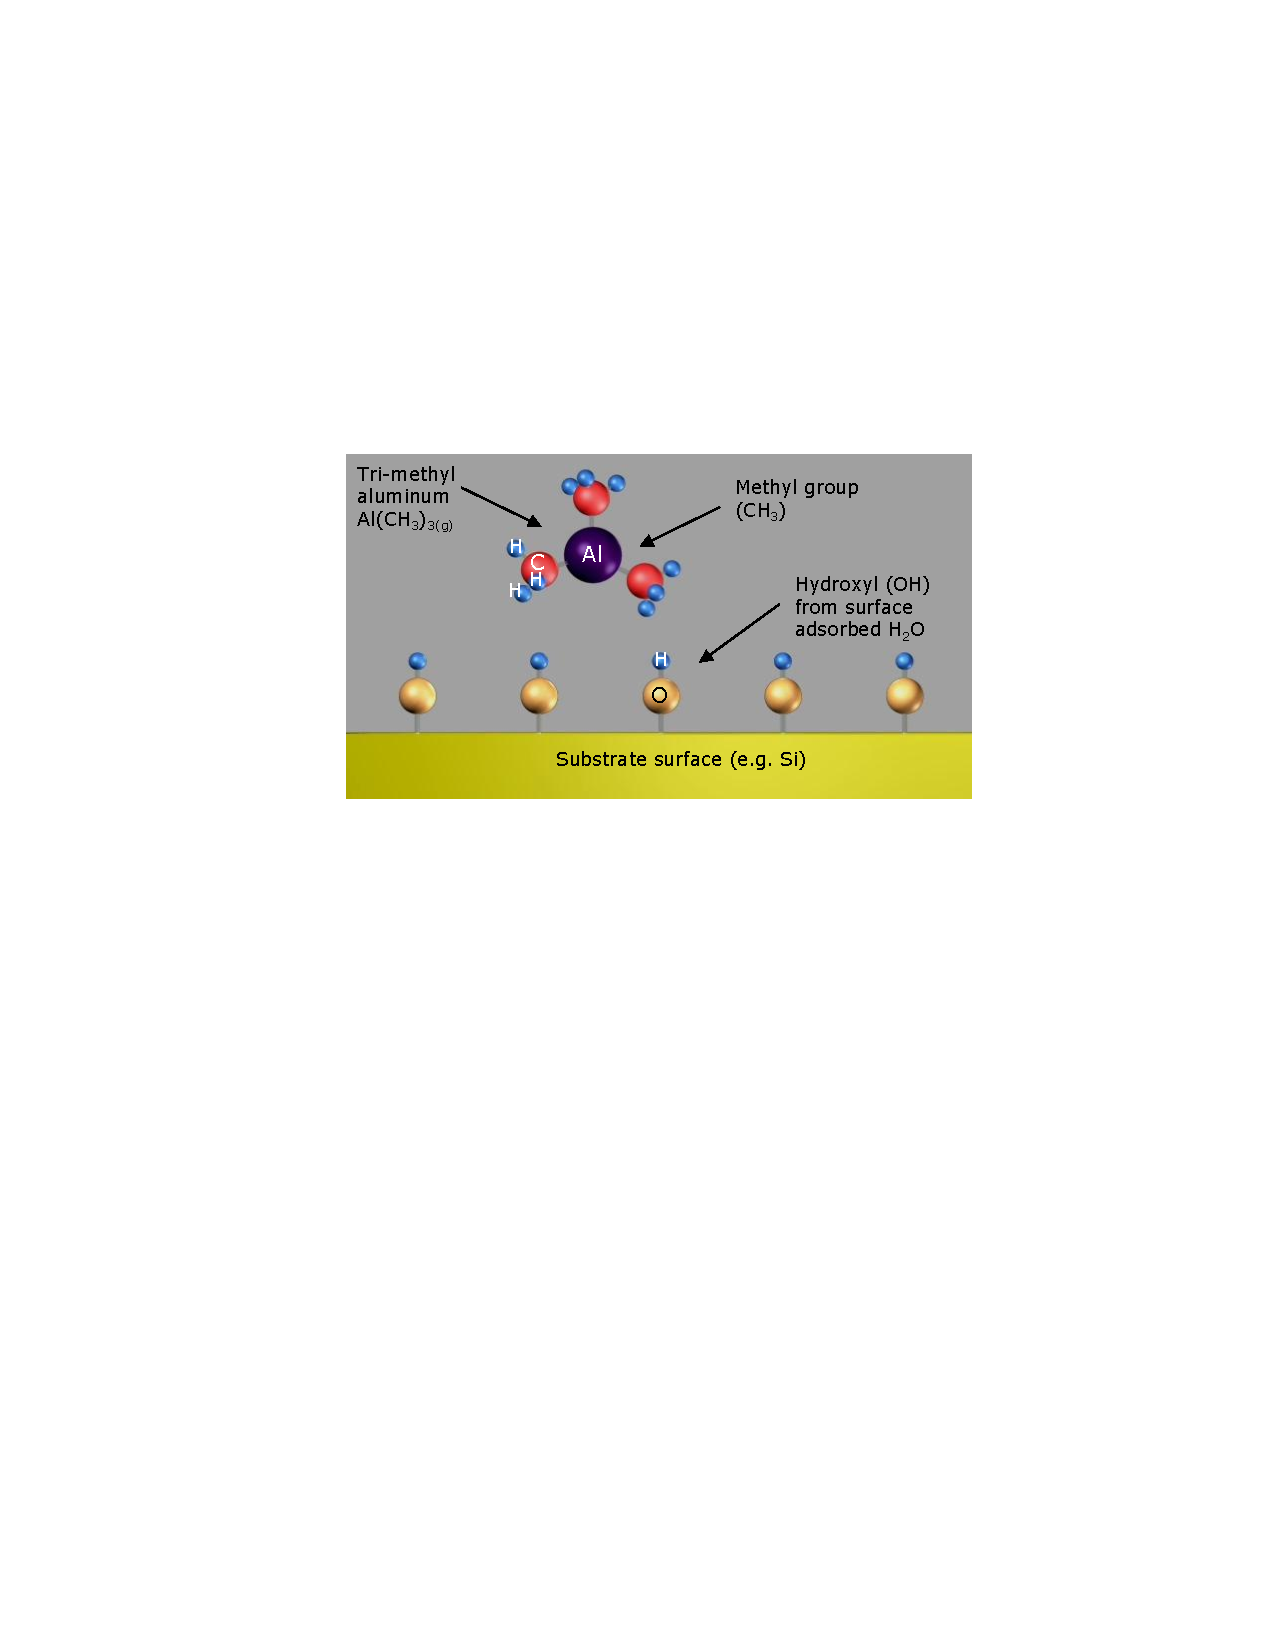
\includegraphics[width=0.9\textwidth]{./Graphics/Synthesis/TMA1}}
		\onslide<2>\centerline{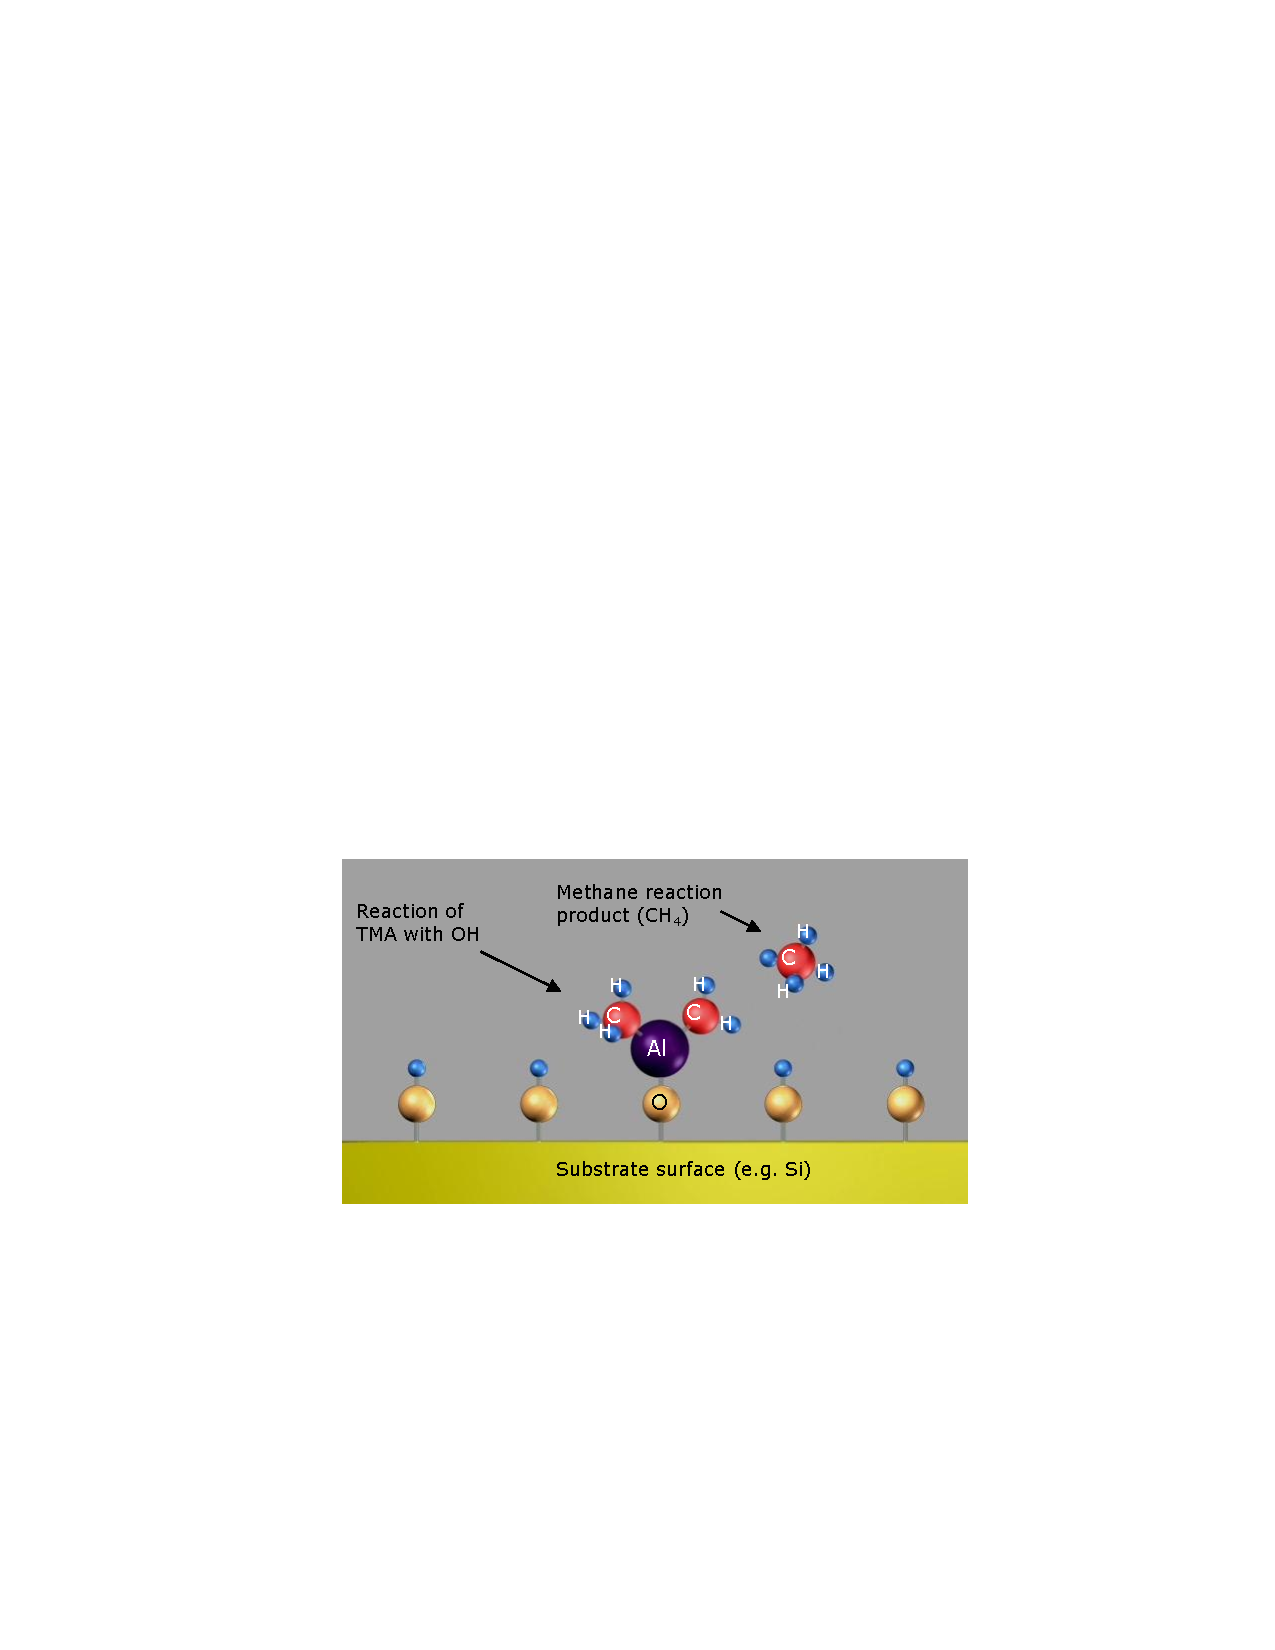
\includegraphics[width=0.9\textwidth]{./Graphics/Synthesis/TMA2}}
		\onslide<3>\centerline{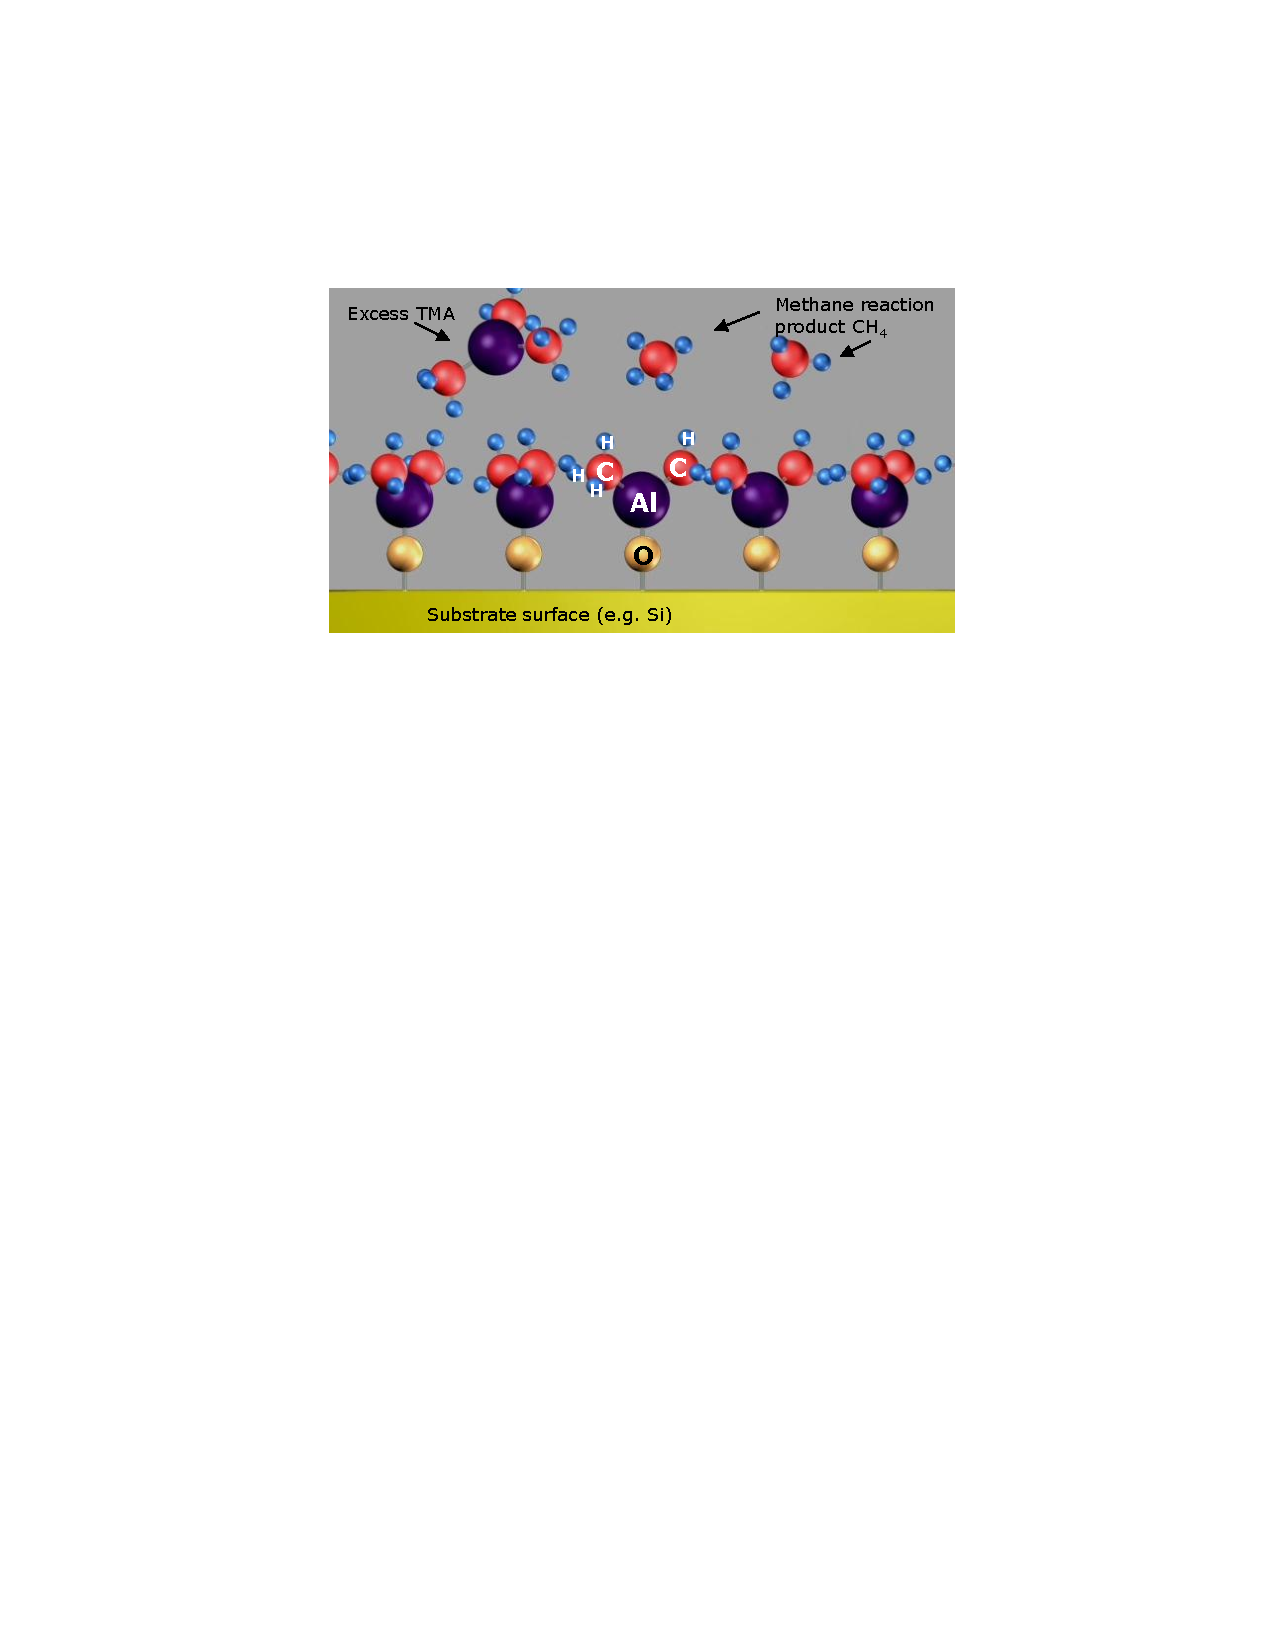
\includegraphics[width=0.9\textwidth]{./Graphics/Synthesis/TMA3}}
		\onslide<4>\centerline{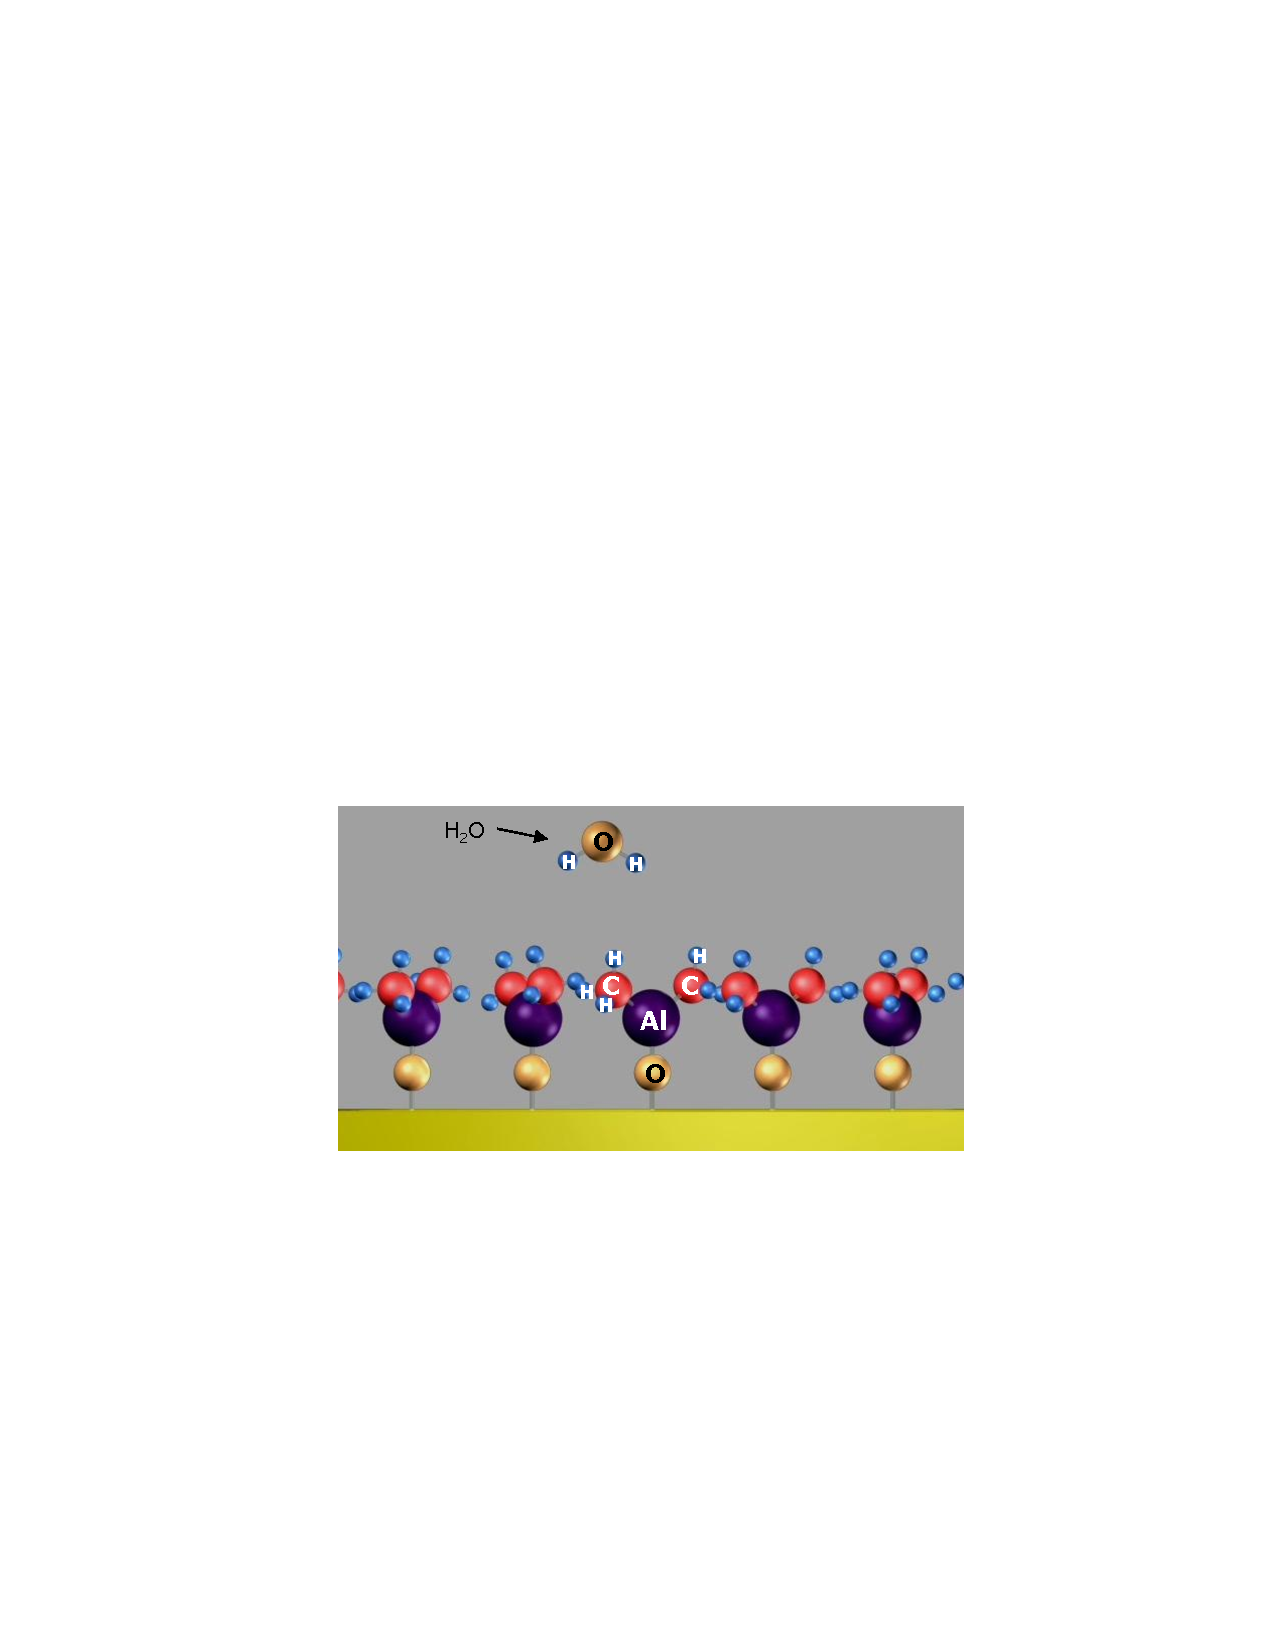
\includegraphics[width=0.9\textwidth]{./Graphics/Synthesis/TMA4}}
		\onslide<5>\centerline{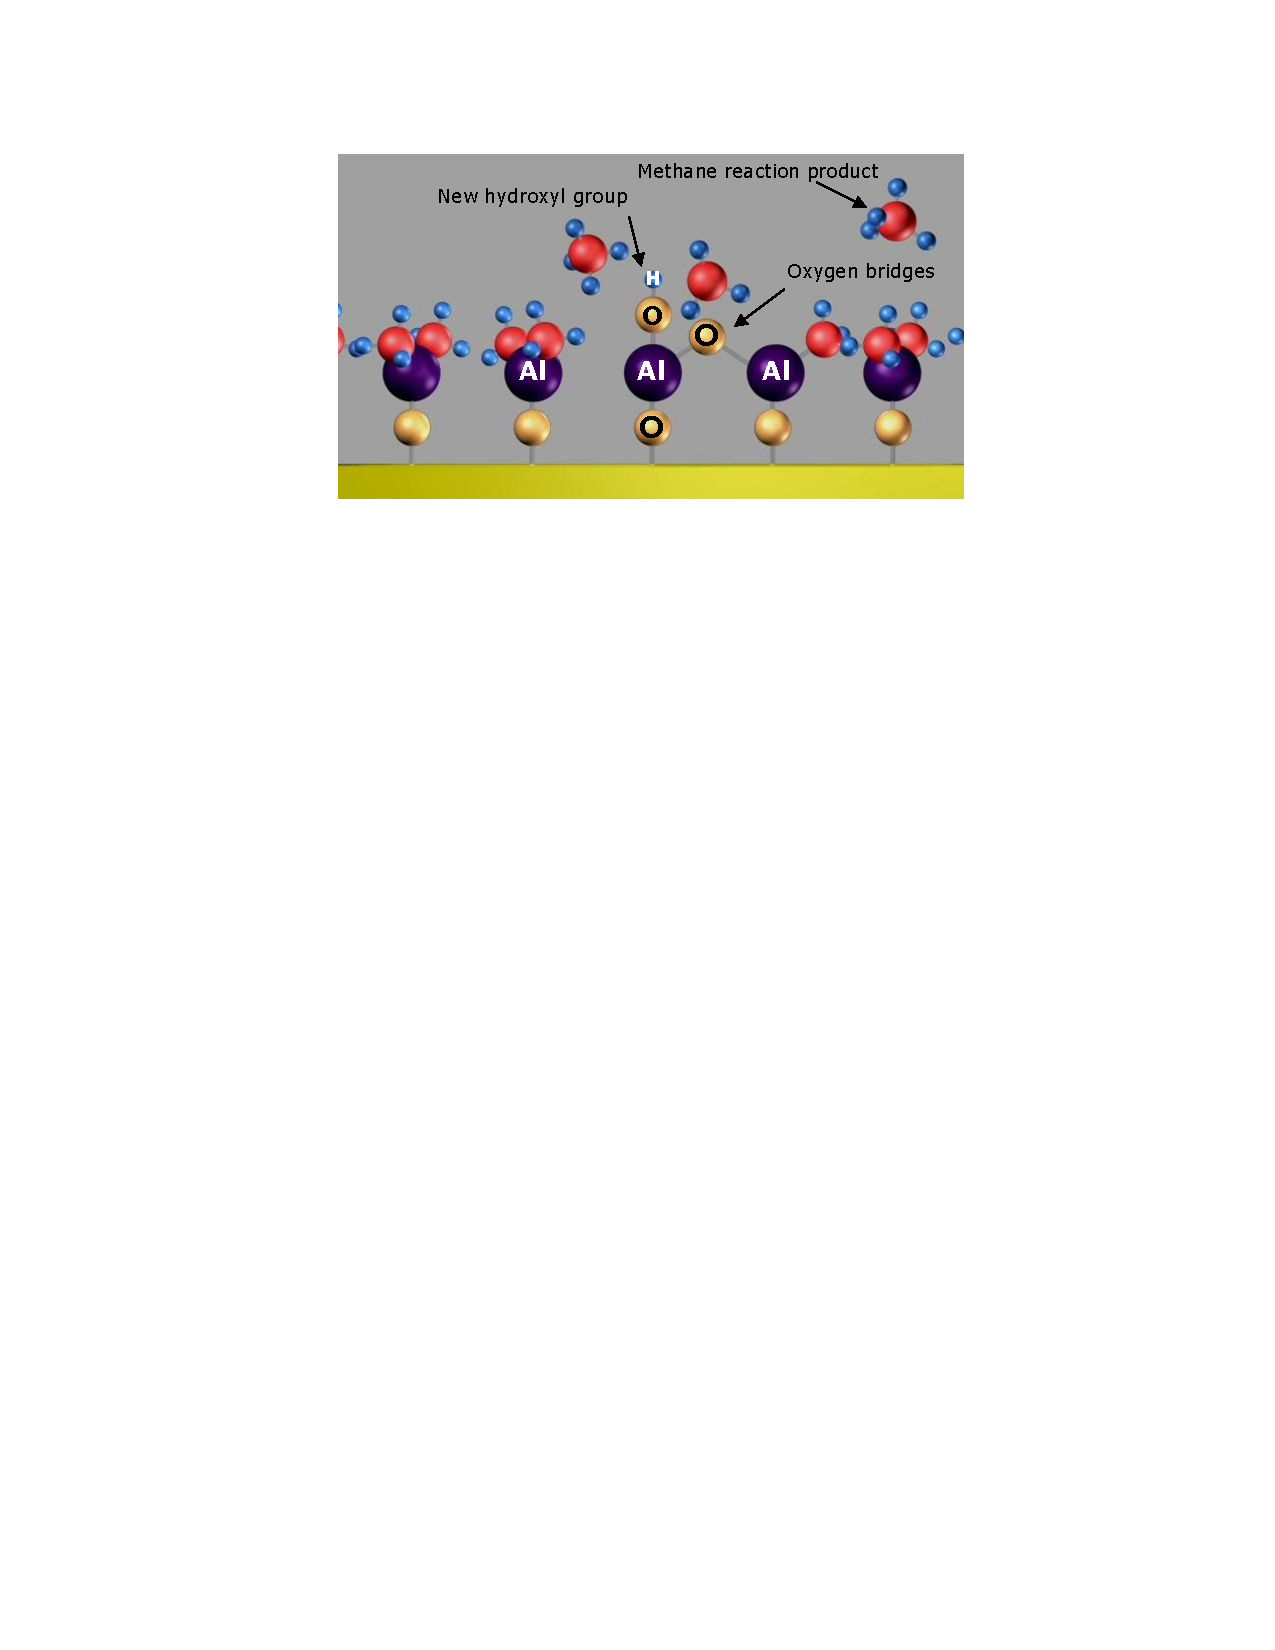
\includegraphics[width=0.9\textwidth]{./Graphics/Synthesis/TMA5}}
		\onslide<6>\centerline{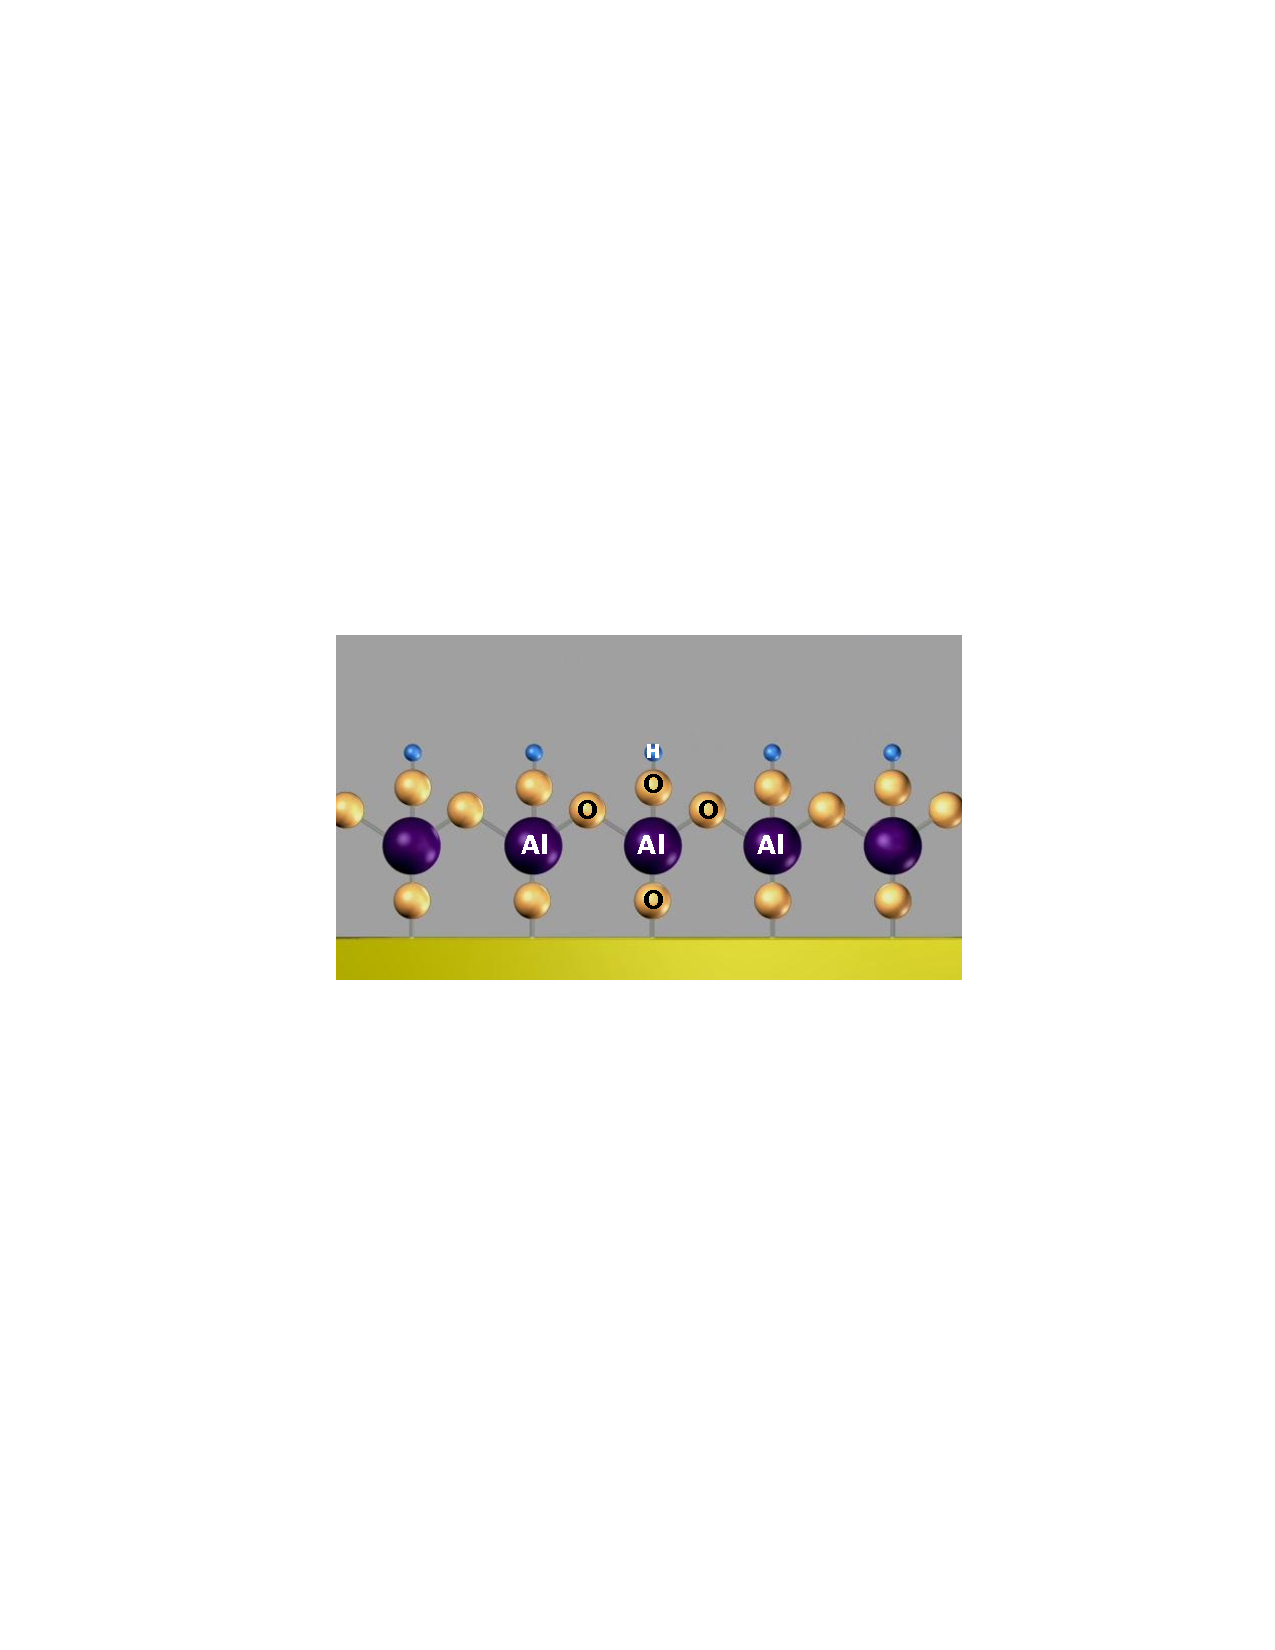
\includegraphics[width=0.9\textwidth]{./Graphics/Synthesis/TMA6}}
	\end{overprint}
\end{frame}

\begin{frame}{Atomic Layer Deposition}
	\vspace{-0.5cm}
	\begin{columns}[t]
		\column{0.5\textwidth}
			\begin{block}{Advantages}
				\begin{itemize}
					\item Ultra-high film thickness resolution (\AA-level)
					\item High film conformality\\(3D structure coating)
					\item Lower deposition temperatures
					\item Potentially lower environmental/economic impact
				\end{itemize}
			\end{block}
		\column{0.5\textwidth}
			\begin{block}{Disadvantages}
				\begin{itemize}
					\item Slow deposition rates
					\item Precursor chemistry is often difficult and complex (organometallic compounds)
					\item Many material systems lack developed ALD processes
				\end{itemize}
			\end{block}
	\end{columns}
\end{frame}

\begin{frame}{Atomic Layer Deposition}
	Where is ALD used?\vspace{1.5em}
	\begin{itemize}%[<+->]
		\item Integrated Circuits: Transistor Gate Oxides (high-k)\vspace{1.5em}
		\item Alternative Energy: Low tolerances for layer thickness, high film uniformity across surface
		\vspace{1.5em}
		\item Biomedical: Uniform coating of highly porous structures
	\end{itemize}
\end{frame}

%%%%%%%%%%%%%%%%%%%%%%%

\section{Thin Film Growth}

\subsection{Film Precursors}
\begin{frame}{Thin Film Growth: Film Precursors}
	\begin{columns}[c]
		\column{0.5\textwidth}
			\begin{block}{Titanium Precursor}
				Titanium(IV) tetraisopropoxide: {Ti-o-\emph{i} -Pr}
			\end{block}
			\vspace{0.5em}
			\begin{block}{Oxidizer}
				\begin{itemize}
					\item \ce{H2O} and \ce{O2}/\ce{O3} mixtures commonly used in literature
					\item \ce{O2}/\ce{O3} was chosen for higher compatibility with Pb precursors
				\end{itemize}
			\end{block}
		\column{0.5\textwidth}
			\begin{block}{Lead Precursors}
				\begin{enumerate}
					\item Bis(2,2,6,6-tetramethyl -3,5-heptanedionato) Lead(II): Pb(TMHD)$_{2}$
					\item Lead(II) hexafluoro- acetylacetonate: Pb(HFAc)$_{2}$
				\end{enumerate}
			\end{block}
	\end{columns}
\end{frame}

\subsection{Deposition Parameters}
\begin{frame}{Thin Film Growth: Deposition Parameters}
\begin{itemize}
	\large
	\item Growth Temperature
	\vspace{1.5em}
	\item Precursor Dosage
	\vspace{1.5em}
	\item Purge Time
	\vspace{1.5em}
	\item Precursor Exposure
	\vspace{1.5em}
	\item Post-Deposition Annealing
	\end{itemize}
\end{frame}

%%%%%%%%%%%%%%%%%%%%%%%

\section{Characterization Methods}

\subsection{Thermal Analysis}
\begin{frame}
	\vspace{-0.5cm}
	\frametitle{Characterization Methods: Thermal Analysis}
	\begin{columns}[t]
		\column{0.5\textwidth}
			\begin{block}{Thermogravimetric Analysis}
				\begin{itemize}
					\item Method for analyzing mass loss rates as function of temperature
					\item Useful for determining optimal evaporation temperatures
					\item Can indicate multi-step evaporation/chemical conversion
				\end{itemize}
			\end{block}
		\column{0.5\textwidth}
			\begin{block}{Differential Calorimetry}
				\begin{itemize}
					\item Allows insight into energetic transformations as a function of temperature
					\item Indicates phase changes, evaporation energies, and structural changes
					\item Useful for analyzing the stability of precursors at desired temperatures
				\end{itemize}
			\end{block}
	\end{columns}
\end{frame}

\subsection{Composition Analysis}
\begin{frame}{Characterization Methods: Composition Analysis}

\begin{overprint}
	\onslide<1>%
		\vspace{0.5cm}
		\textbf{\large X-Ray Fluorescence Spectroscopy (XRF)}\vspace{1.5em}
		\begin{itemize}
			\item Similar to EDXS but uses X-rays in place of energetic electrons\vspace{1.5em}
			\item Much lower noise floor (no Bremsstrahlung radiation)\vspace{1.5em}
			\item Capable of quantitative compositional analysis of ultra-thin films
		\end{itemize}
	\onslide<2>\vspace{-0.5cm}\centerline{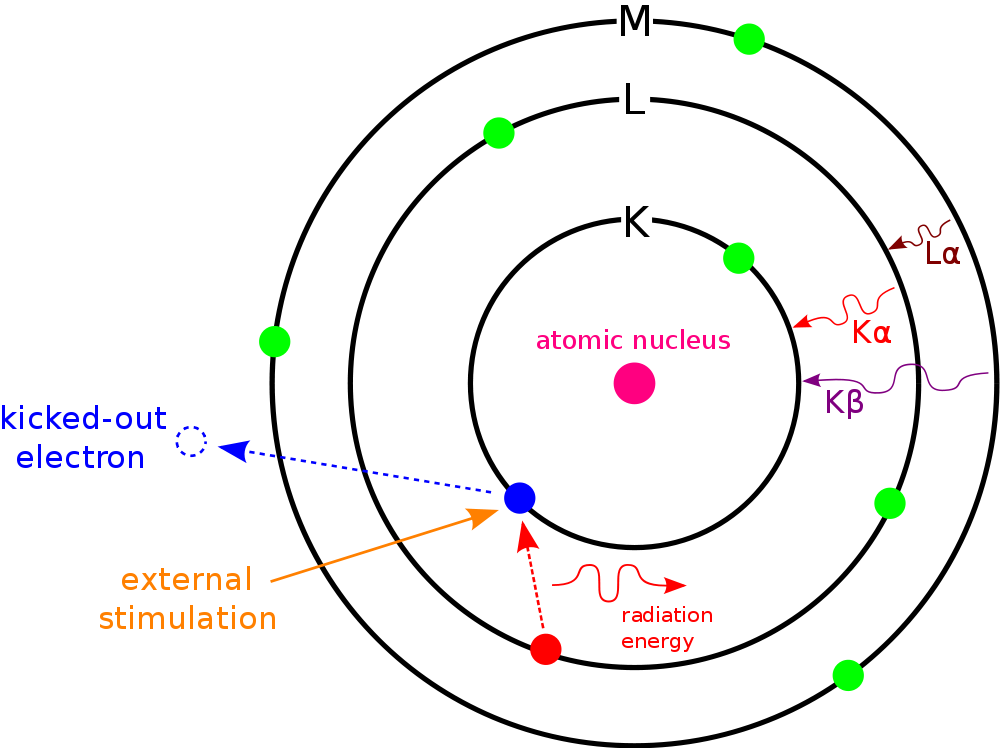
\includegraphics[width=0.9\textwidth]{./graphics/characterization/EDXS-scheme}}
\end{overprint}

\end{frame}

\subsection{Film Growth Rates}
\begin{frame}{Characterization Methods: Film Growth Rates}
\begin{overprint}
	\onslide<1>
		\vspace{0.5cm}
		\textbf{\large Ellipsometry}\vspace{1.5em}
		\begin{itemize}
			\item Non-destructive optical film analysis method\vspace{1.5em}
			\item Capable of determining numerous optical/electronic parameters of film\vspace{1.5em}
			\item Primarily used to determine post-deposition film thicknesses and thus growth rates
		\end{itemize}
	\onslide<2>
		\centerline{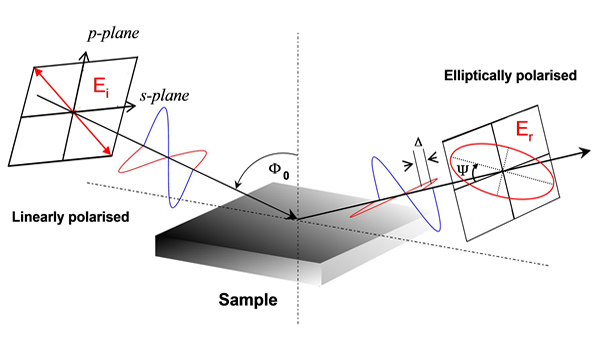
\includegraphics[width=\textwidth]{./graphics/characterization/ellipsometryDiagram_simple}}
\end{overprint}
\end{frame}

\subsection{Phase Identification}
\begin{frame}{Characterization Methods: Phase Identification}

\textbf{\large X-Ray Diffractometry (XRD)}
\vspace{1.5em}
\begin{itemize}
	\item Standard technique used to identify materials and phases/orientations
	\vspace{1.5em}
	\item Analysis produces information about presence of particular lattice spacings
	\vspace{1.5em}
	\item Identifying lattice spacings (via databases or previous studies in literature) can indicate presence and orientation of specific materials and phases 
\end{itemize}

\end{frame}

%%%%%%%%%%%%%%%%%%%%%%%

\section{Results}

\subsection{Thermal}
\begin{frame}{Results: Thermal Analysis}
\begin{overprint}
	\onslide<1>
		\begin{center}
		TGA Traces for \ce{Pb(HFAc)2}\\
		\vspace{0.5cm}
		\centerline{\includegraphics[width=\textwidth]{./graphics/data/tga/hfac}}
		\end{center}
	\onslide<2>
		\begin{center}
		TGA Traces for \ce{Pb(TMHD)2}\\
		\vspace{0.5cm}
		\centerline{\includegraphics[width=\textwidth]{./graphics/data/tga/tmhd}}
		\end{center}
	\onslide<3>
		\begin{center}
		Constant Temperature Studies of \ce{Pb(HFAc)2} and \ce{Pb(TMHD)2}\\
		\vspace{0.5cm}
		\centerline{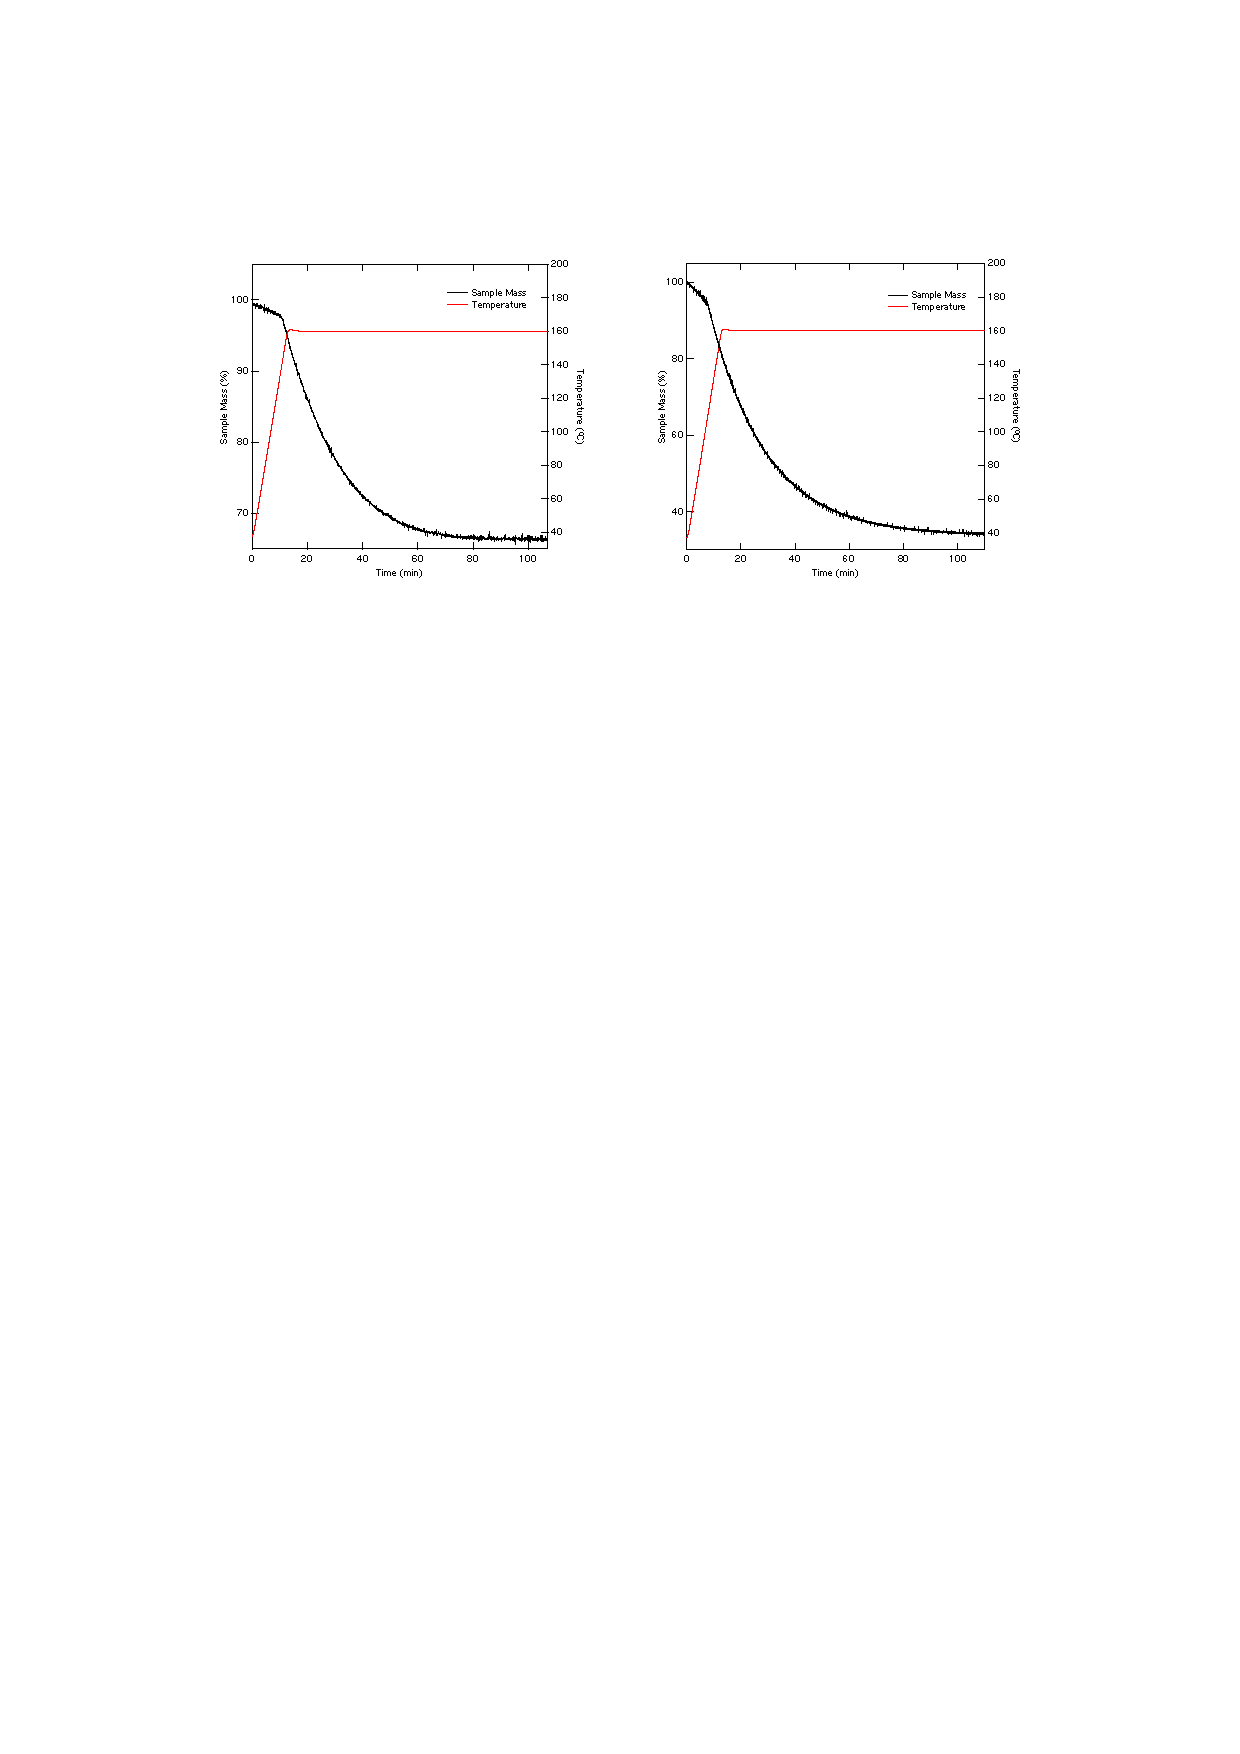
\includegraphics[width=\textwidth]{./graphics/data/tga/hold}}
		\end{center}
	\onslide<4>
		\begin{center}
%		\vspace{-0.5cm}
		DSC Cycles of \ce{Pb(HFAc)2} and \ce{Pb(TMHD)2}\\
		\vspace{0.5cm}
		\centerline{\includegraphics[width=0.45\textwidth]{./graphics/data/dsc/hfac}%
			\hspace{0.5cm}%
			\includegraphics[width=0.45\textwidth]{./graphics/data/dsc/tmhd}}
		\end{center}
		
\end{overprint}
\end{frame}

\subsection{Film Growth}
\begin{frame}{Results: Film Growth Rates}
\centerline{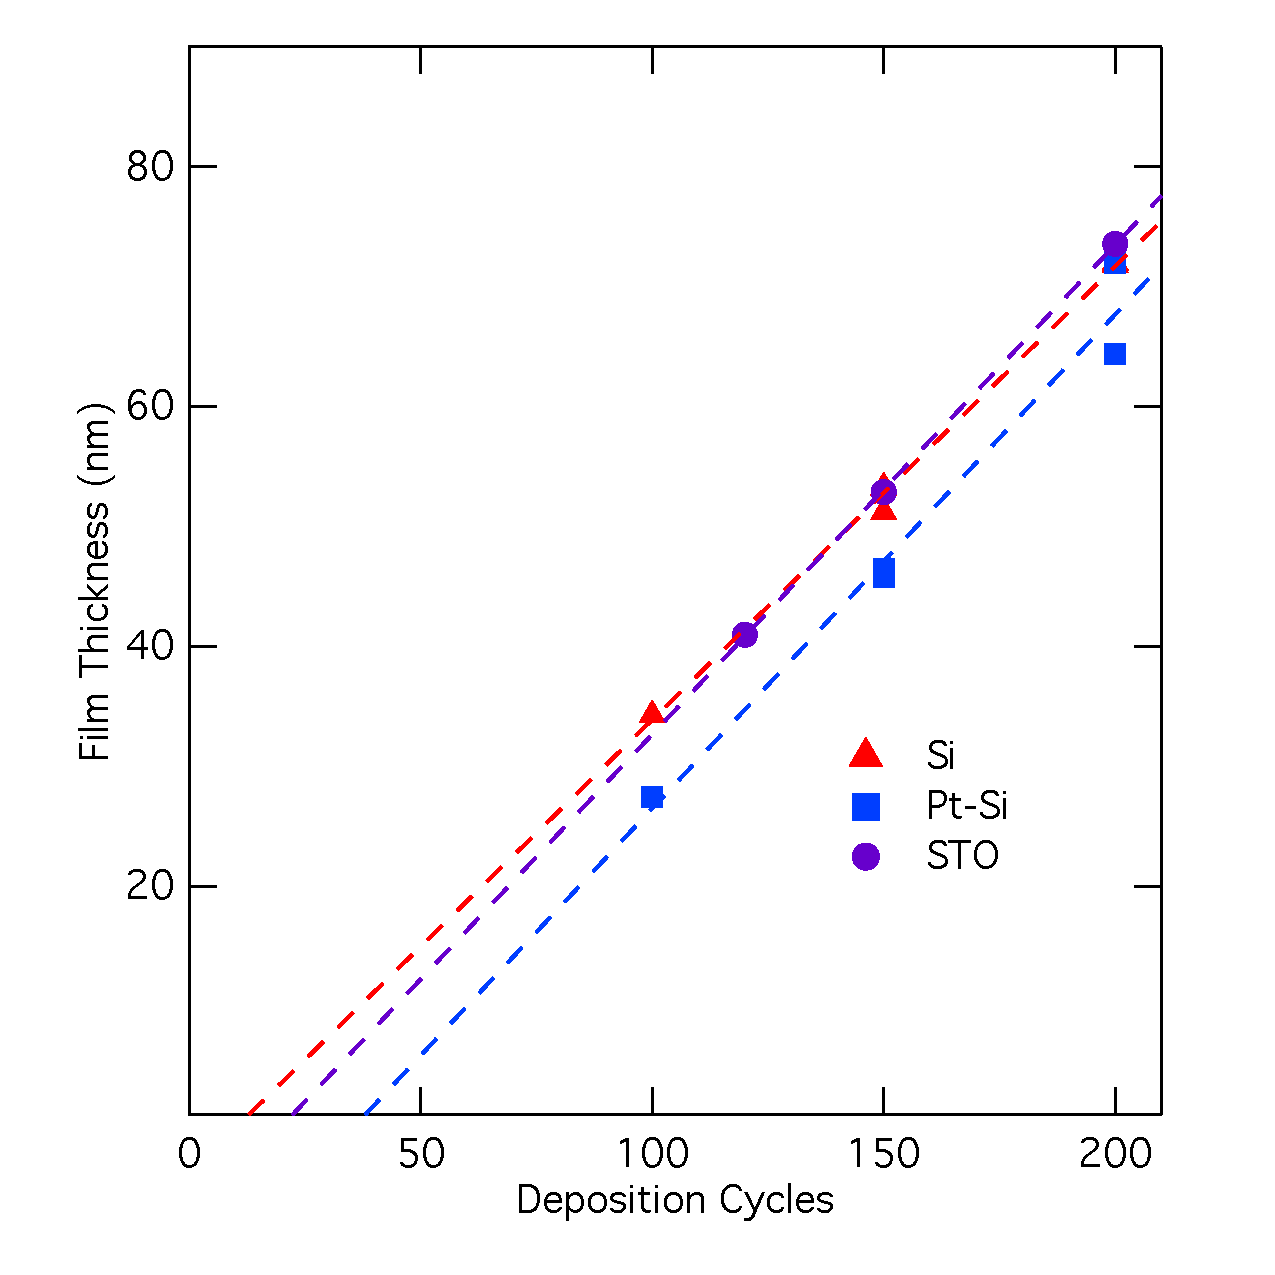
\includegraphics[width=0.7\textwidth]{./graphics/data/ellipsometry/Ellip-Rates}}
\end{frame}

\subsection{Composition Analysis}
\begin{frame}{Results: Composition Analysis}
	\small
	\begin{center}
	\vspace{-0.5cm}
	Compositions of Selected Sample Films\\\vspace{0.5em}
	\begin{tabular}{l l r r r}
	\toprule
	&&\multicolumn{3}{c}{Composition (\%)}\\
	\cmidrule{3-5}
	Run \#&Substrate&Lead&Titanium&Ti:Pb Ratio\\
	\midrule
% 	Run	Sub-Type		Pb%		Ti%		Ti:Pb ratio
	19	&\ce{SiO2}	&65.9	&34.1	&0.518\\
		&Pt-Si		&42.9	&57.1	&1.333\\
	20	&\ce{SiO2}	&56.6	&43.4	&0.769\\
		&Pt-Si		&51.5	&48.5	&0.944\\
	21	&\ce{SiO2}	&69.6	&30.4	&0.437\\
		&Pt-Si		&56.1	&43.9	&0.783\\
	22	&\ce{SiO2}	&67.7	&32.3	&0.478\\
		&Pt-Si		&56.1	&43.9	&0.784\\
	23	&\ce{SiO2}	&66.9	&33.1	&0.495\\
		&Pt-Si		&49.1	&50.9	&1.038\\
	24	&\ce{SiO2}	&69.0	&31.0	&0.450\\
		&Pt-Si		&62.2	&37.8	&0.609\\
	\bottomrule
	\end{tabular}
	\end{center}
\end{frame}

\subsection{Phase Identification}
\begin{frame}{Results: Phase Identification}
\begin{overprint}
	\onslide<1>
		\begin{center}
		\textbf{\Large XRD of 20 on Pt-Si}\vspace{0.25cm}
		\centerline{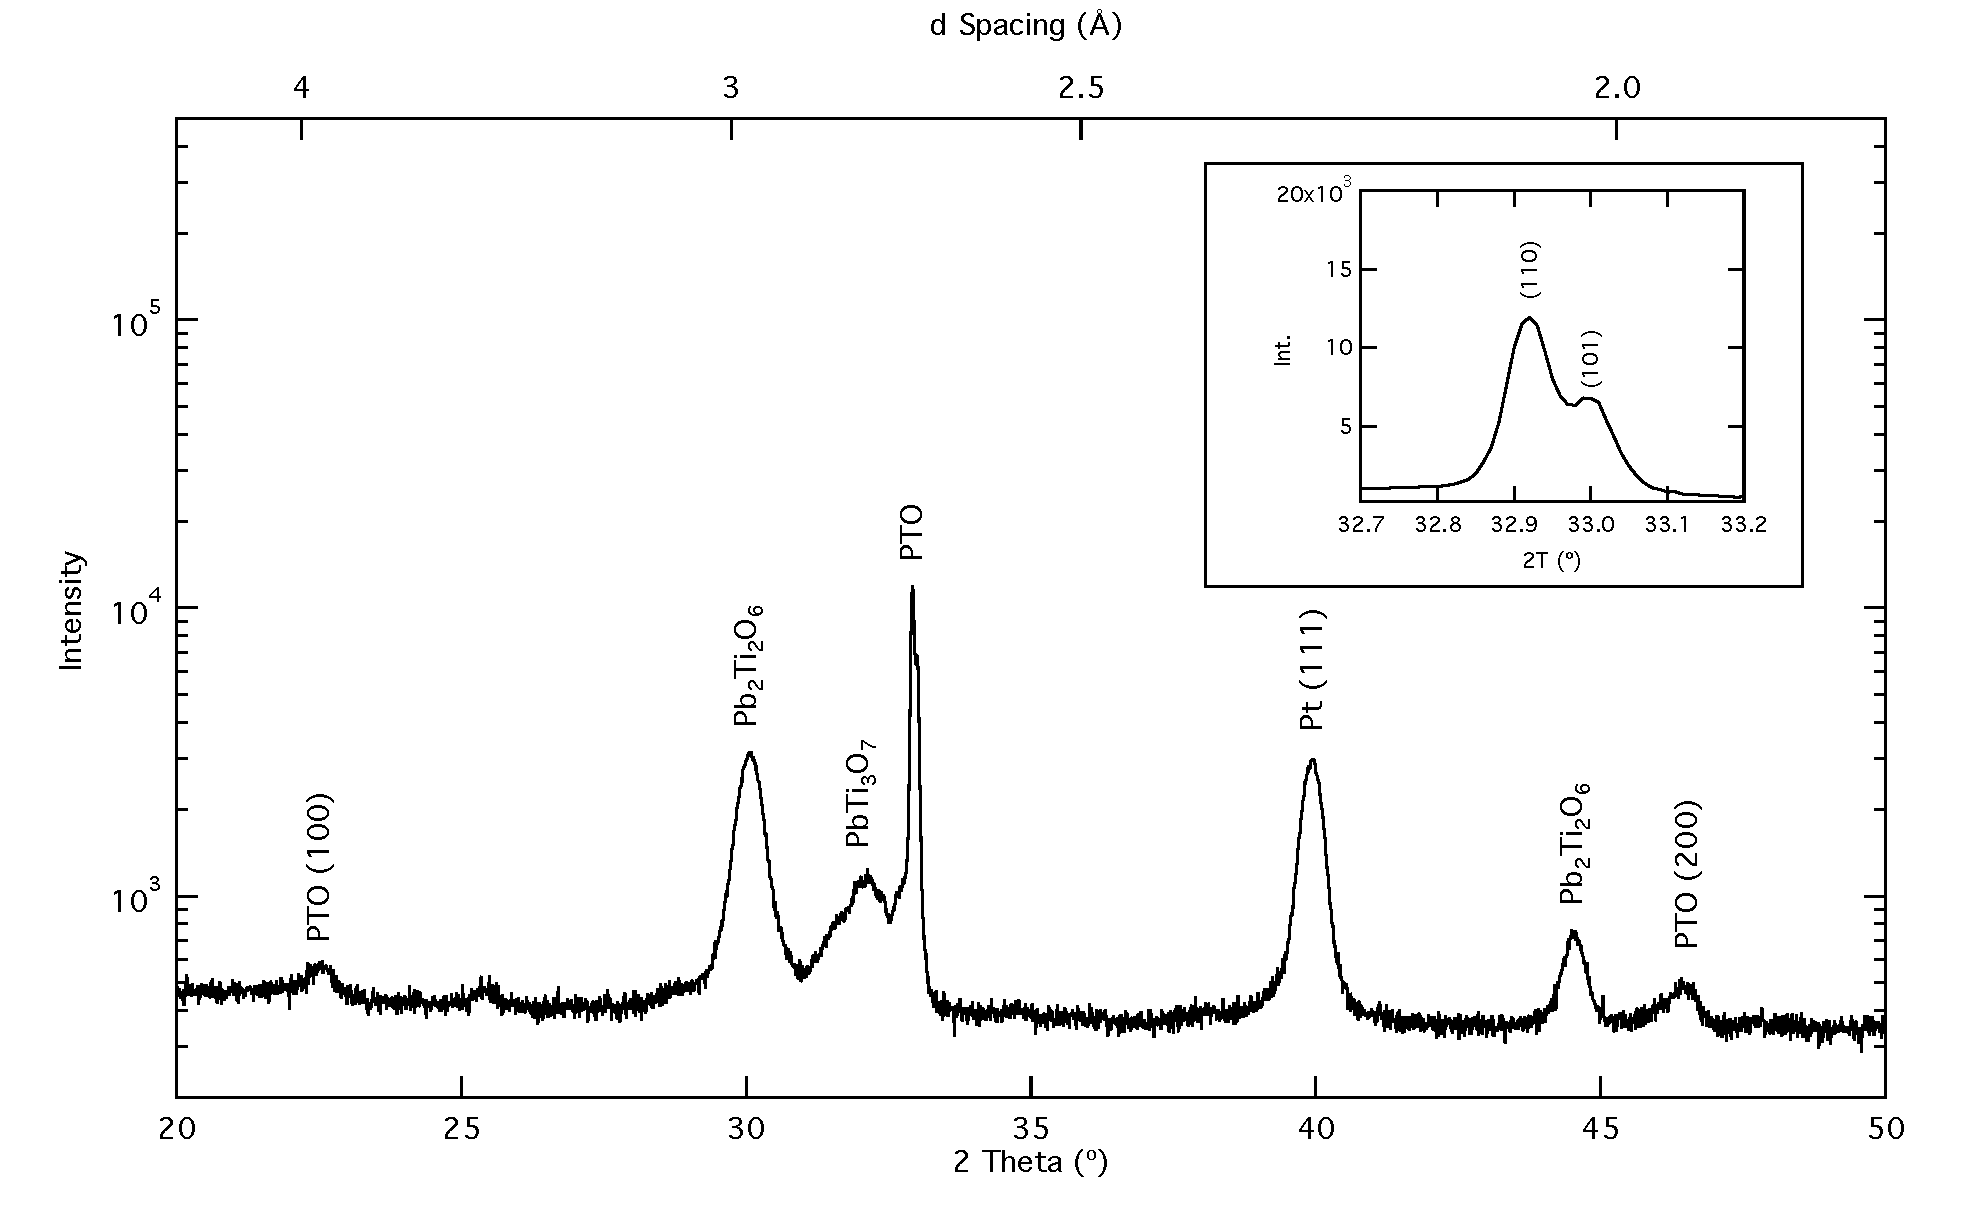
\includegraphics[width=\textwidth]{./graphics/data/xrd/20Pt}}
		\end{center}
	\onslide<2>
		\begin{center}
		\textbf{\Large XRD of 23 on Pt-Si}
		\centerline{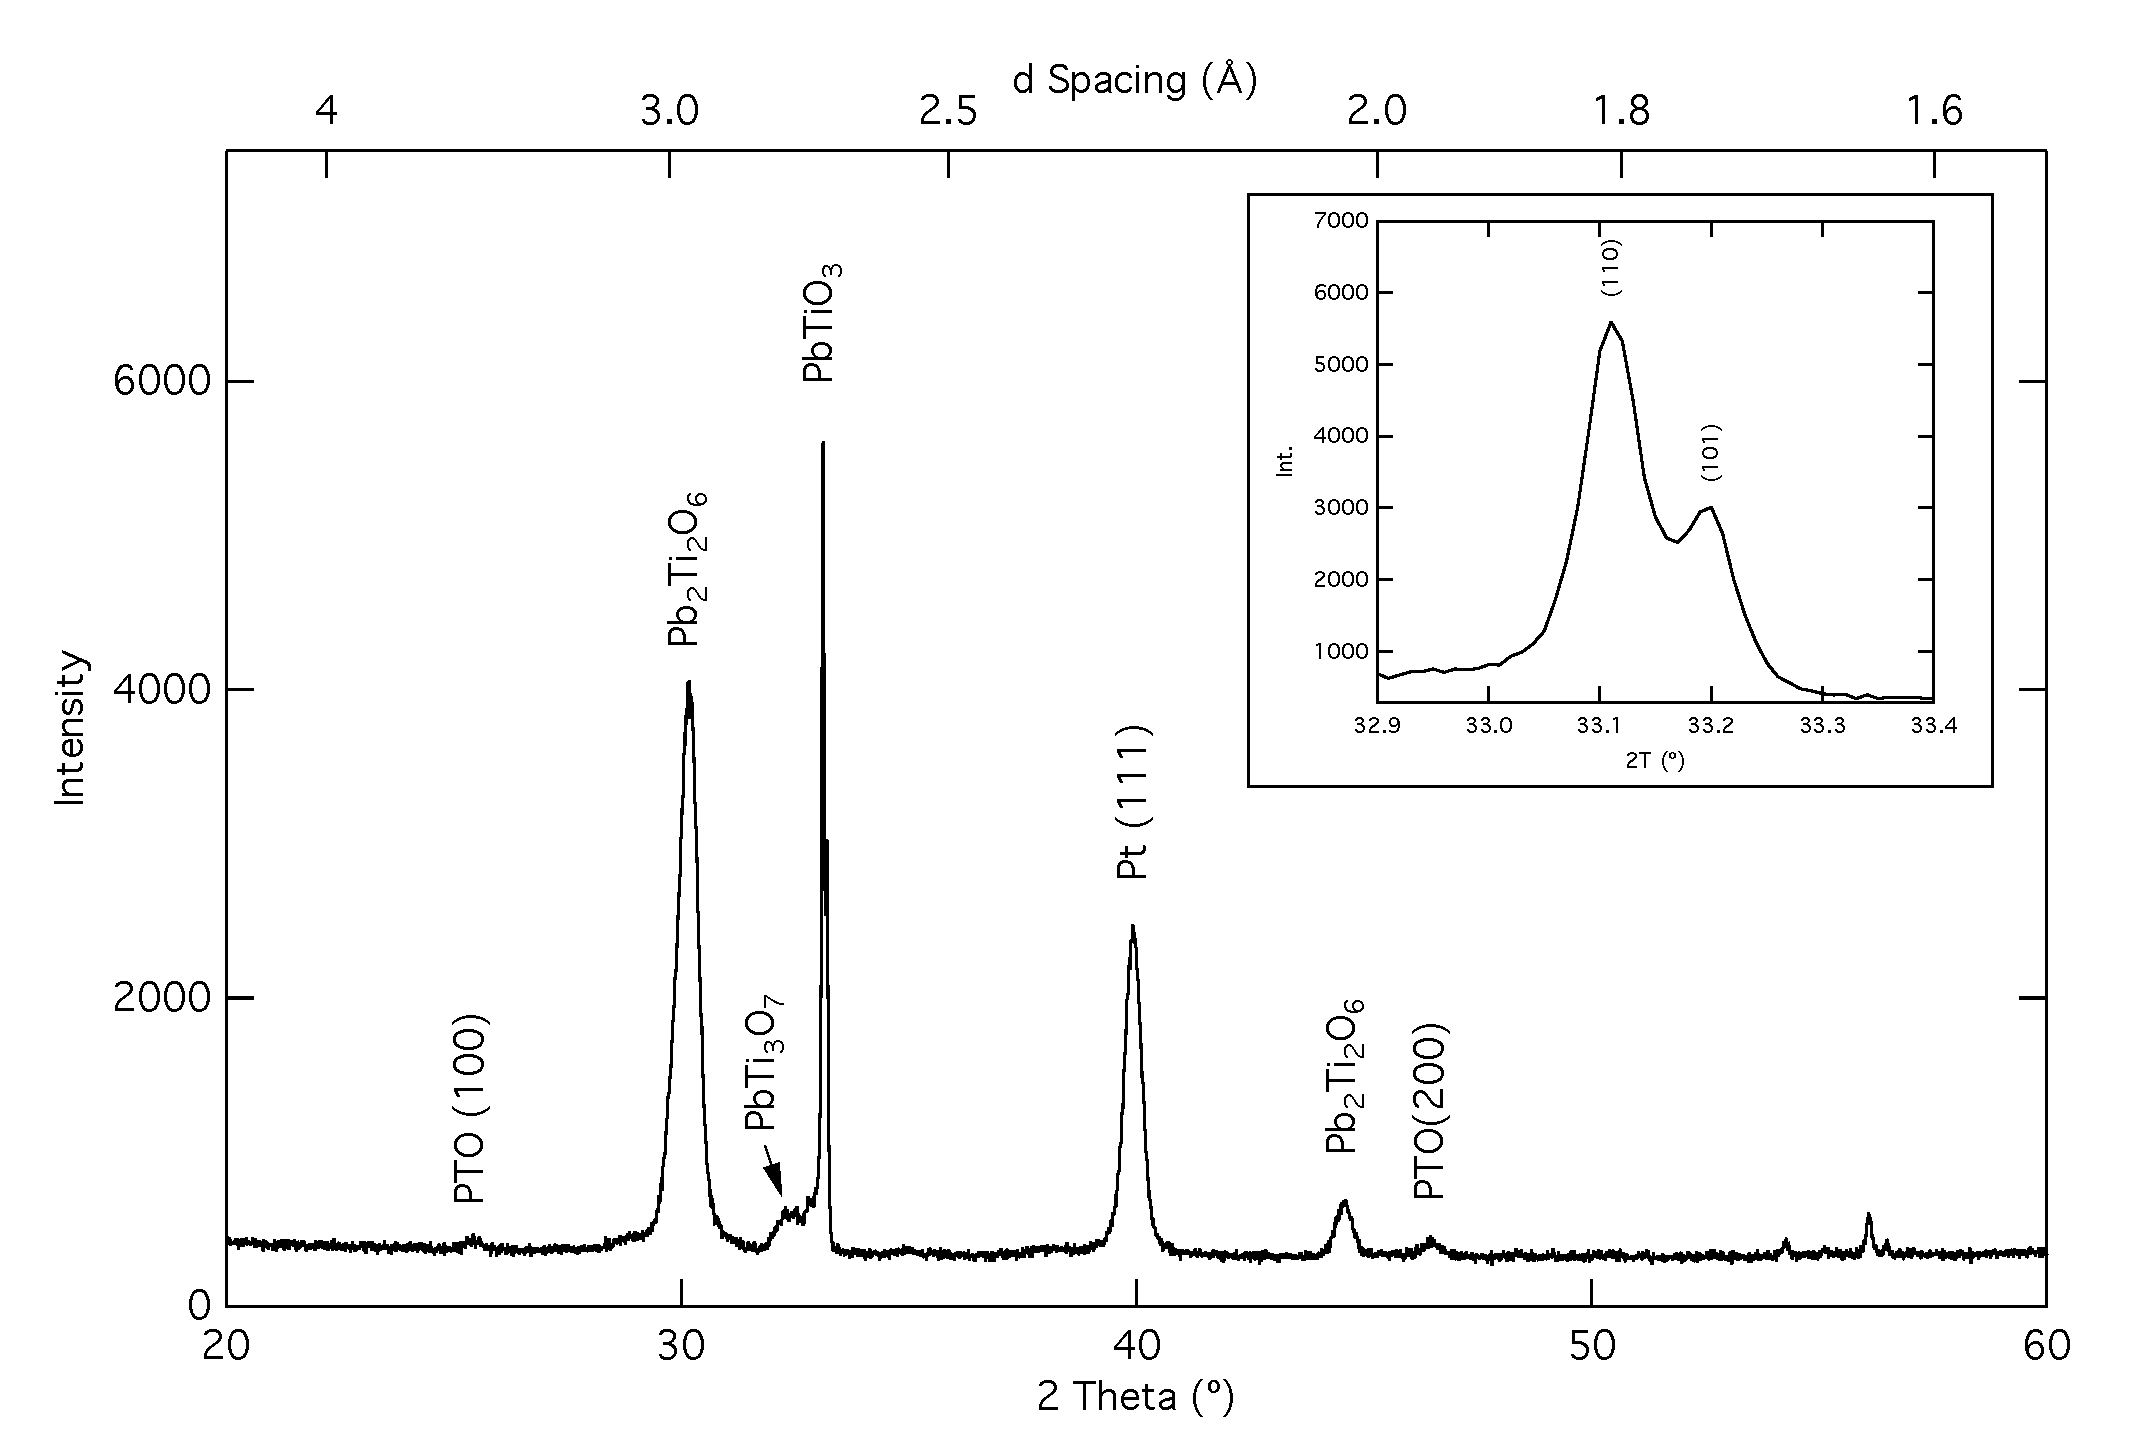
\includegraphics[width=0.95\textwidth]{./graphics/data/xrd/23Pt}}
		\end{center}
	\onslide<3>
		\begin{center}
		\textbf{\Large XRD of 28 on STO(100)}
		\centerline{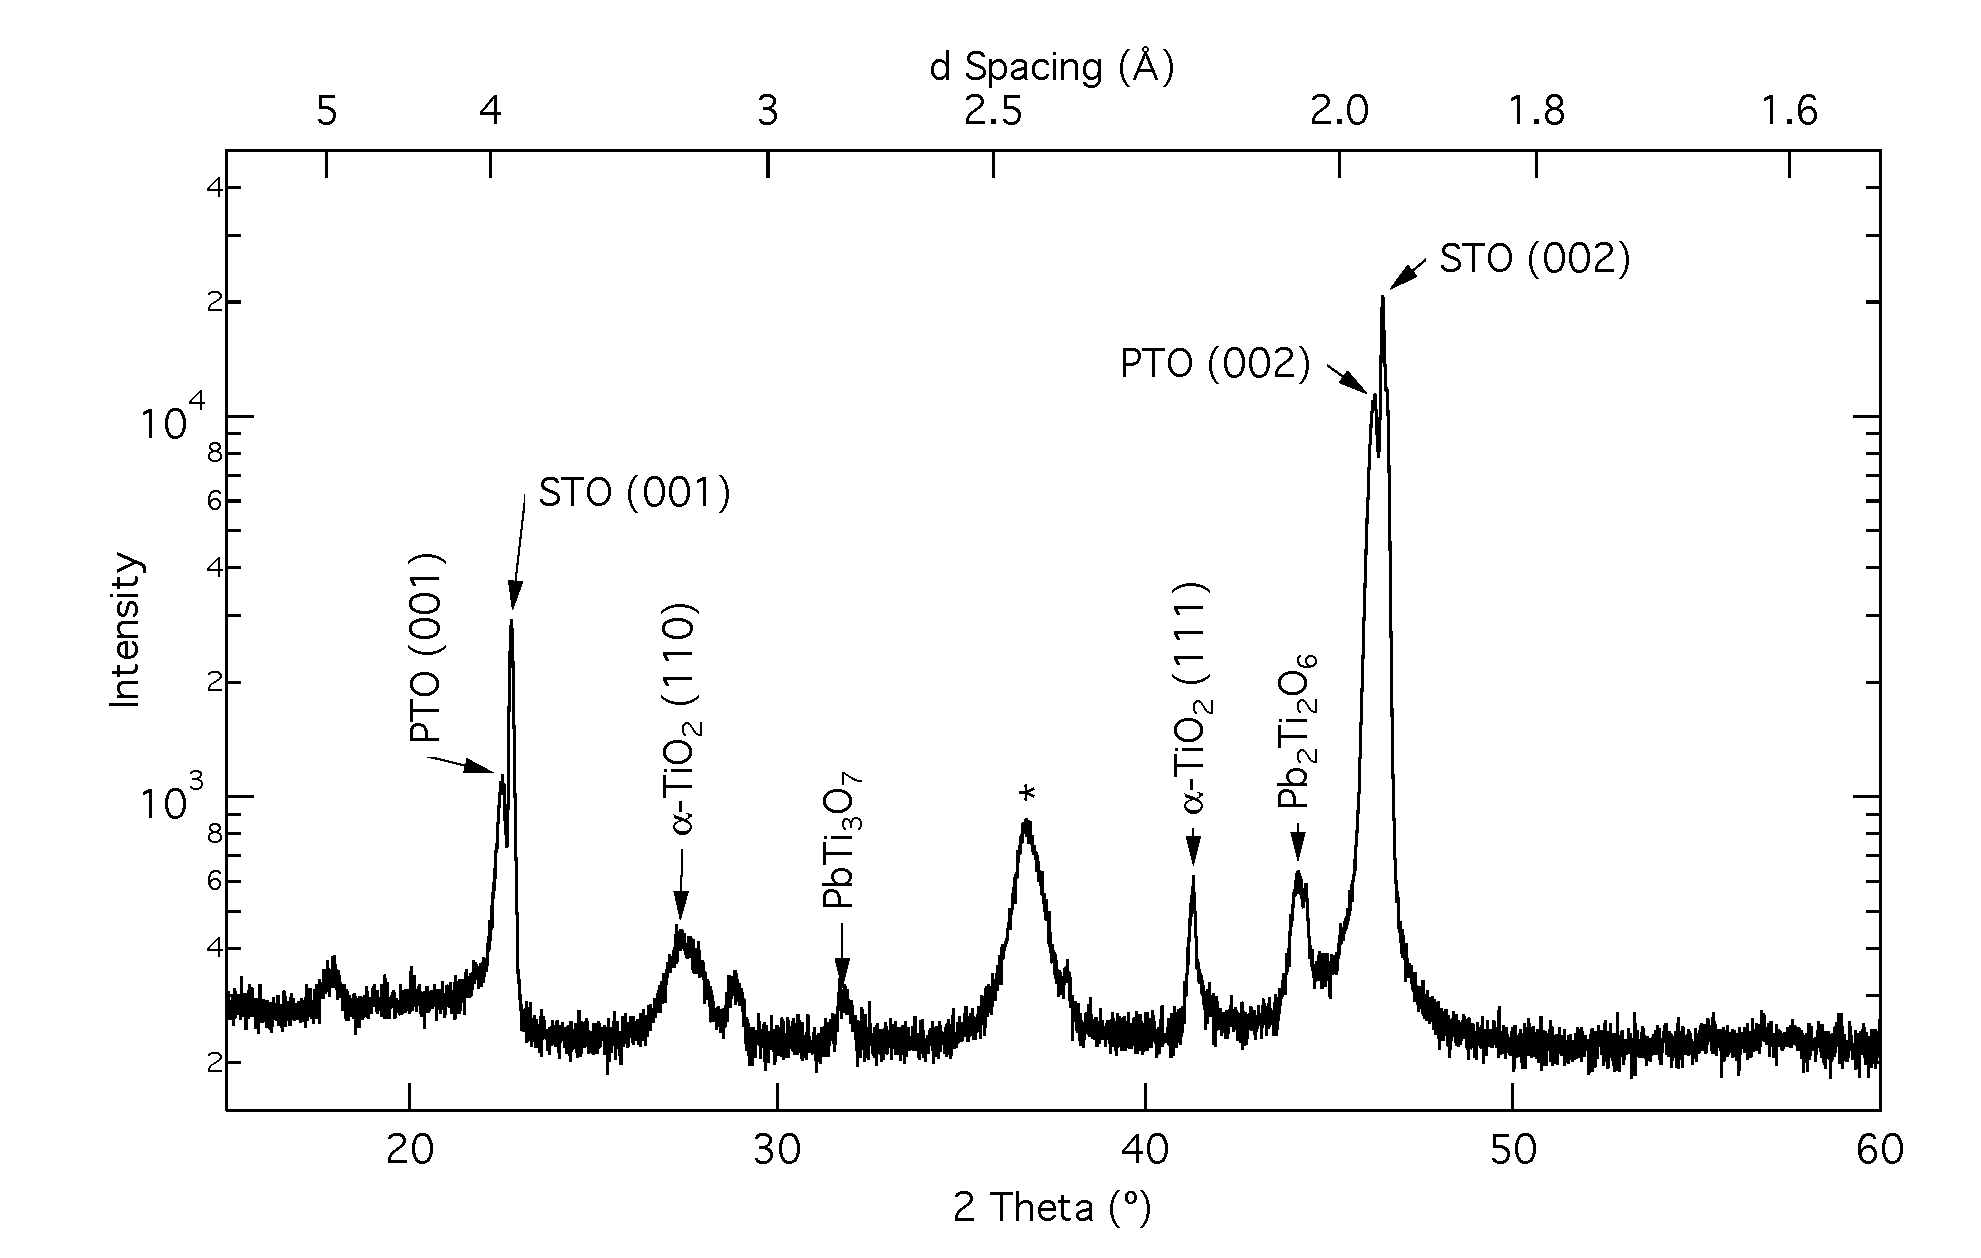
\includegraphics[width=\textwidth]{./graphics/data/xrd/28STO}}
		\end{center}
\end{overprint}
\end{frame}

%%%%%%%%%%%%%%%%%%%%%%%

\section{Conclusions}

\begin{frame}{Conclusions}

\begin{itemize}
\item A method for designing and implementing an ALD process for a novel material has been developed
\vspace{1.5em}
\item Successfully deposited thin films containing the target material: perovskite \ce{PbTiO3}
\vspace{1.5em}
\item Films contain significant amounts of impurity phases
\end{itemize}
\end{frame}

\subsection{Future Work}
\begin{frame}{Conclusions: Future Work}
\begin{itemize}
\item Refine process to maximize phase purity and film epitaxy
\vspace{2em}
\item Characterize ferroelectric character of crystallized films
\vspace{2em}
\item Investigate doping of thin films (e.g. \ce{PbZr_{x}Ti_{1-x}O3})
\vspace{2em}
\item Apply process to other oxide families (e.g. \ce{BaSrTiO3})
\end{itemize}
\end{frame}

%%%%%%%%%%%%%%%%%%%%%%%

\begin{frame}
	\vfill
	\begin{center}
		{\Huge Questions?}
	\end{center}
\end{frame}


\begin{frame}
\end{frame}

\begin{frame}
\end{frame}

\begin{frame}
\end{frame}

\begin{frame}
\end{frame}



\end{document}












